\subsection{Broad Comparison With the Same Validation Population}
The broader study (Study A) asks a different question from the earlier RSR 12~dB,
three-to-seven-path comparison: how well do the frozen methods work
across the full noise/reference/path grid used for validation? OptShrink
receives the same validation observations and selection loss as the
learned estimator, with a larger classical search. No test-channel
labels select its settings.

\begin{table*}[!t]
\caption{Broad comparisons on separate fresh banks. Study A tests offline tuning; Study B adds online rank selection on a new bank. Each study has 4,032 primary worlds and 64 excluded stress worlds. Lower NMSE is better. Times use the same PyTorch CPU backend and include selection/refitting. Learned metrics average three frozen models, not an ensemble.}
\label{tab:broad}\centering\footnotesize
\setlength{\tabcolsep}{4pt}
\begin{tabular}{@{}lrrrr@{}}\toprule
Method & A: NMSE (dB) & Time (ms) & B: NMSE (dB) & Time (ms)\\
\midrule
Compact estimator (188 weights) & -13.565 & 4.90 & -13.647 & 4.96\\
Offline OptShrink, selected placement & -13.028 & 15.61 & -13.196 & 15.76\\
Offline OptShrink, in-loop & -13.000 & 15.57 & -13.151 & 15.68\\
Offline OptShrink, final-only & -12.827 & 6.16 & -12.863 & 6.23\\
Online rank + placement selection & --- & --- & -14.096 & 114.17\\
Online rank, in-loop & --- & --- & -14.154 & 108.70\\
Online rank, final-only & --- & --- & -13.723 & 13.96\\
HS-Rician, one sweep & -12.996 & 98.91 & -13.059 & 99.88\\
EM-GS, 100 updates & -9.922 & 13.08 & -9.958 & 13.15\\
\bottomrule
\end{tabular}
\end{table*}


The compact estimator reaches $-13.565$~dB, compared with $-13.028$~dB
for the validation-selected OptShrink placement. The gain is
0.537~dB, with adjusted 95\% interval $[0.450,0.695]$~dB. It also
gains 0.565~dB over separately tuned in-loop OptShrink and 0.738~dB
over final-only OptShrink. Table~\ref{tab:broad} reports all principal
controls. Every original learned seed has a lower primary average
than the selected classical control; seed-specific scores range from
$-13.327$ to $-13.692$~dB. These are three fitted models from one
training dataset, not three independent training populations.

The benefit is uneven. Learning wins in 79 of 126 cells. Averaging
over noise and reference levels, it gains 2.190~dB for two paths but
loses 0.272~dB for sixteen paths. Its worst primary-cell loss is
3.117~dB, at SNR 20/RSR 20~dB with sixteen paths. These results do
not erase the earlier few-path losses against different controls.
They show why the comparator, tuning population and averaging rule
must be stated together.

Mean processing time is 4.90~ms for the compact estimator, 15.61~ms
for selected OptShrink and 6.16~ms for final-only OptShrink. A
separately tuned ten-update OptShrink control takes 4.56~ms and
reaches $-12.336$~dB. Thus the learned model is not the fastest tested
choice, but improves accuracy over that similar-cost control. These
times count inference only; the neural model needs offline training
and OptShrink needs offline tuning. The complete broad comparison,
including tuning, testing, timing and audit, took about 71 minutes.
That is not a separate measurement of tuning cost.

The headline gain also depends on error aggregation. Pooling linear
errors across all primary worlds before taking dB reduces the gain
to 0.116~dB. The learned estimator has fewer errors above NMSE one
(3.03\% versus 4.34\%), but more above 0.5 (19.54\% versus 19.12\%).
No errors above two occur for these two methods in this sample; this
does not establish zero risk. In the excluded weak-reference check,
learning loses 4.063~dB. At SNR 60~dB it reaches $-6.693$~dB, whereas
selected OptShrink reaches $-66.886$~dB. The broader average supports
a useful operating-range comparison, not reliable behavior outside it.

\subsection{What Changes When OptShrink Selects Rank Online?}
Study B uses 4,096 further fresh worlds. The compact estimator reaches
$-13.647$~dB on the primary average. Online in-loop OptShrink reaches
$-14.154$~dB, improving on learning by 0.507~dB, with adjusted 95\%
interval $[0.437,0.562]$~dB. Joint rank-and-placement selection reaches
$-14.096$~dB and improves on learning by 0.449~dB, with interval
$[0.358,0.569]$~dB. Final-only rank selection reaches $-13.723$~dB;
its 0.076~dB point advantage has interval $[-0.025,0.226]$~dB.
That interval establishes neither superiority nor equivalence.

The in-loop selector is therefore the strongest tested method on
this primary accuracy measure. The joint selector was declared in
advance and is reported even though searching more choices did not
give the lowest test error. Rician prediction loss on nine withheld
pilots is not a channel-error guarantee, and restarting on all pilots
changes the fitted estimate. We do not identify either effect as the
sole cause of the observed ranking.

The cost is substantial in this implementation: mean times are
108.70~ms for online in-loop selection, 114.17~ms for joint selection,
13.96~ms for final-only selection and 4.96~ms for the compact model.
All candidate fitting and all-pilot refitting are included. Inference
is about 22 times faster for the learned model than for online in-loop
selection under this single-thread, batch-one test. This ratio does
not include amortized training cost and is not a prediction for other
devices, batch sizes or optimized implementations.

Learning has fewer primary errors above NMSE one: 3.08\%, compared
with 6.87\% for online in-loop and 5.78\% for joint selection. At
threshold 0.5, learning has 19.55\% exceedances, compared with
19.52\% and 19.22\%, respectively. Thus the primary accuracy winner
and the winner at one severe-error threshold differ. Neither
method's settings were selected to minimize that error frequency,
and these observations are not communication-outage probabilities.

Pooling linear errors across primary worlds also favors learning:
its pooled NMSE is $-6.683$~dB versus $-6.217$~dB for online in-loop
selection. This descriptive difference does not replace the declared
average-cell-dB result. The former is more influenced by large errors;
the latter gives each operating cell equal weight in dB.

The limits remain large. The compact model's worst primary-cell loss
to the in-loop selector is 5.495~dB. Joint selection also beats it in
the weak-reference stress case ($-10.101$ versus $-7.787$~dB) and
the nearly noiseless case ($-70.134$ versus $-6.835$~dB). These
failures remain outside the primary average but inside the report.
The final result supports a measured accuracy--cost trade-off; it
does not support the claim that our estimator beats tuned OptShrink
once observation-based rank selection is allowed.


\begin{figure*}[!t]
\centering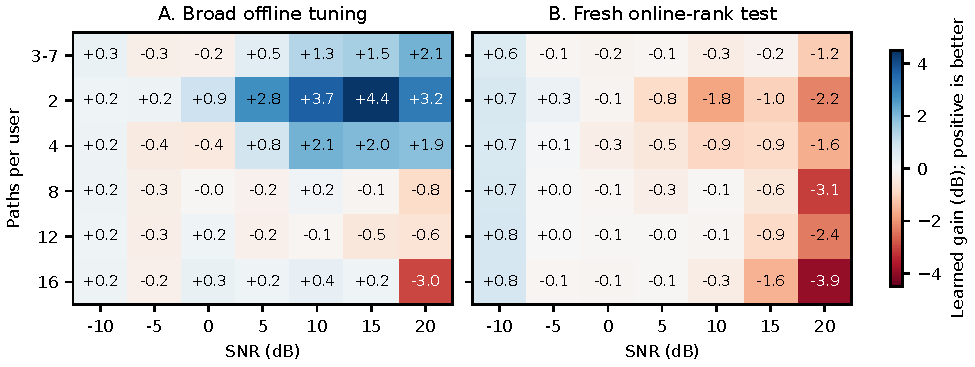
\includegraphics[width=\textwidth]{latest_gains.pdf}
\caption{Learned gain over (a) broad offline-selected OptShrink and
(b) online in-loop rank selection on a separate fresh bank.
Positive values favor learning. Each square averages three RSR-specific
cell dB gains; the random 3--7 row draws path counts independently for
each user. These descriptive averages are not cellwise confidence
guarantees. The full individual-cell values are retained in the evidence
records.}
\label{fig:broad-gains}
\end{figure*}

The failed extensions are also relevant. A corrected learned gate around
OptShrink gains only 0.019~dB over its strong starting baseline and
loses to retuned classical mixing and a simpler stage-only learned
rule. Simple stopping/filter-release rules do not improve their
primary average. A small-budget exact-EM Transformer run is worse
than EM100 and is not a strong URformer comparison. These separate
pilots do not support replacing the original compact estimator or
claiming a new improved OptShrink algorithm. Their results and the
failed local error-model screen are retained in the supplement.
